% Packages
\documentclass[12pt]{article}
\usepackage[margin=2.5cm]{geometry}
\usepackage{lipsum}
\usepackage{titlesec, titletoc}
\usepackage[svgnames, table]{xcolor}
\usepackage{algorithm}
\usepackage{algpseudocode}
\usepackage{mdframed}
\usepackage[T1]{fontenc}
\usepackage{amsmath,amsthm,amsfonts,amssymb,mathtools}
\usepackage[osf]{mathpazo}
\usepackage{enumitem}

% Formating setup
\footskip = 1 cm
\setlength{\parindent}{0pt}
\pdfpxdimen=1in
\parindent = 0pt
\definecolor{myBlue}{RGB}{0, 81, 255}
\titleformat{\section}[block]{\sffamily\large\bfseries}{\thesection}{.5em}{\textcolor{myBlue}
{\titlerule[1.5pt]}\\\sffamily}[\vspace*{-3mm}\textcolor{myBlue}{\titlerule[1.5pt]}]
\titleformat{\subsection}{\large\sffamily\bfseries}{\thesubsection}{0.5em}{\textcolor{Black}}
\newcounter{boxedlistcounter}
\newenvironment{pseudo}{%
  \setcounter{boxedlistcounter}{0}% <-- Add this line to reset the counter
  \mdframed[
    linecolor=black, % color of the border
    linewidth=1.5pt, % thickness of the border
    roundcorner=10pt, % radius of the corners
    innertopmargin=0.6\baselineskip, % space at the top of the box
    innerbottommargin=0.6\baselineskip, % space at the bottom of the box
  ]
  \fontsize{12pt}{14pt}\selectfont % add font size command here
  \mdseries % add font series command here
}{%
  \endmdframed%
}
\newcommand{\I}{\par\stepcounter{boxedlistcounter}\arabic{boxedlistcounter}.\hspace{5pt}}
\newcounter{boxedlistcounter2}
\newenvironment{Proof}{%
  \refstepcounter{boxedlistcounter2}%
  \mdframed[
    linecolor=black, % color of the border
    linewidth=1.5pt, % thickness of the border
    roundcorner=10pt, % radius of the corners
    innertopmargin=\baselineskip, % space at the top of the box
    innerbottommargin=\baselineskip, % space at the bottom of the box
  ]
  \fontsize{12pt}{14pt}\selectfont % add font size command here
  \mdseries % add font series command here
}{%
  \endmdframed%
}
\newcommand{\PI}{\par\textbullet\hspace{5pt}}
\setlist[itemize]{itemsep=1pt}
\newcommand{\NL}{\par\hspace{12.5pt}}
\setlist[itemize]{itemsep=1pt}

% Custom commands
\newcommand{\for}[1]{\textbf{for} #1 \textbf{do}}
\newcommand{\IF}[1]{\textbf{if} #1 \textbf{then}}
\newcommand{\ELIF}[1]{\textbf{else if} #1 \textbf{then}}
\newcommand{\ELSE}{\textbf{else}}
\newcommand{\return}[1]{\textbf{return} #1}
\newcommand{\assign}{ $\leftarrow$ }
\newcommand{\DEF}[2]{\textbf{def} #1(#2):}
\newcommand{\1}{\space \quad}
\newcommand{\2}{\quad \quad \quad}
\newcommand{\3}{\quad \quad \quad \quad \space}
\newcommand{\4}{\quad \quad \quad \quad \quad \quad}
\newcommand{\5}{\quad \quad \quad \quad \quad \quad \quad \space}
\newcommand{\comment}[1]{\hfill \textit{\# #1}}
\newcommand{\while}[1]{\textbf{while} #1 \textbf{do}}

% Document start ------------------------------------------------------------------------------------
\begin{document}

% Section 1  ----------------------------------------------------------------------------------------
\section{Introduction to Graphs}
A graph G is a pair (V, E), where V is a set of nodes, called vertices and E is a collection of pairs of 
vertices, called edges.

\vspace{10pt}
\textbf{Edge Types}\\
A graph can be directed or undirected. In a directed graph, the edges are ordered pairs of vertices (u, v),
where u is the origin/tail and v is the destination/head. In an undirected graph, the edges are unordered 
pairs of vertices (u,v), whereby u and v can access each other either way.

\vspace{10pt}
\textbf{Simple paths}\\
A path is a sequence/set of vertices such that every pair of consecutive vertices is connected by an edge. A simple
path is a path with no repeated vertices. As such, all vertices in that path are distinct. 

\vspace{10pt}
\textbf{Cycles in graphs}\\
A cycle is a path with at least one edge, whose first and last vertices are the same. A simple cycle is a cycle.
A simple cycle is one where all vertices are distinct, except for the first and last vertices. An acyclic graph has 
no cycle in it, which is impossible for undirected graphs. A directed graph can be acyclic.

\vspace{10pt}
\textbf{Subgraphs}\\
A subgraph S of a graph G is defined as S = (U, F) where U is a subset of vertices in V and F is a subset of edges 
in E. An induced subgraph of G is a subgraph that is formed by selecting a subset U of vertices and all the edges 
in G that have both endpoints in U, which is denoted as G[U]. Similarly, an induced subgraph can be formed by selecting 
a subset F of edges and the vertices that are endpoints of the edges in F, which is denoted as G[F].

\vspace{10pt}
\textbf{Connectivity}\\
A graph G = (V, E) is considered connected if there is a path between every pair of vertices in V. In other words, 
every vertex in the graph is reachable from every other vertex. A connected component of a graph G is a maximally connected 
subgraph of G, meaning that it is a subgraph that is connected, and there is no larger connected subgraph that contains it. 
A graph is considered disconnected if it has two or more connected components, which means that there are pairs of vertices 
that are not connected by any path in the graph.

\vspace{10pt}
\textbf{Trees and Forests}\\
An unrooted tree is a graph that is connected and has no cycles. A forest is a graph without cycles, and its connected components 
are trees. Every tree on n vertices has exactly n-1 edges, which is a well-known property of trees in graph theory. A rooted 
tree is a type of tree that is produced by a directed graph where the edges are directed away from the root.

\subsection{Graph Properties}
\begin{itemize}
  \item $\sum_{v \in V}$ deg(v) = 2m, where m is the number of edges in the graph. This states that the sum of the 
  degrees of all the vertices in the graph is equal to twice the number of edges in the graph.
  \item In a simple undirected graph m <= n (n - 1)/2.
  \item n represents the number of vertices, m represents the number of edges. And $\triangle$ represents the maximum degree.
\end{itemize}

% Section 2  ----------------------------------------------------------------------------------------
\section{Graph ADT}
We model the abstraction as a combination of three data types: Vertex, Edge, and Graph.
A Vertex stores an associated object (e.g., an airport code) that is retrieved with a getElement() method.
An Edge stores an associated object (e.g., a flight number, travel distance) that is retrieved with a getElement() method. 

\subsection{Edge List Structure}
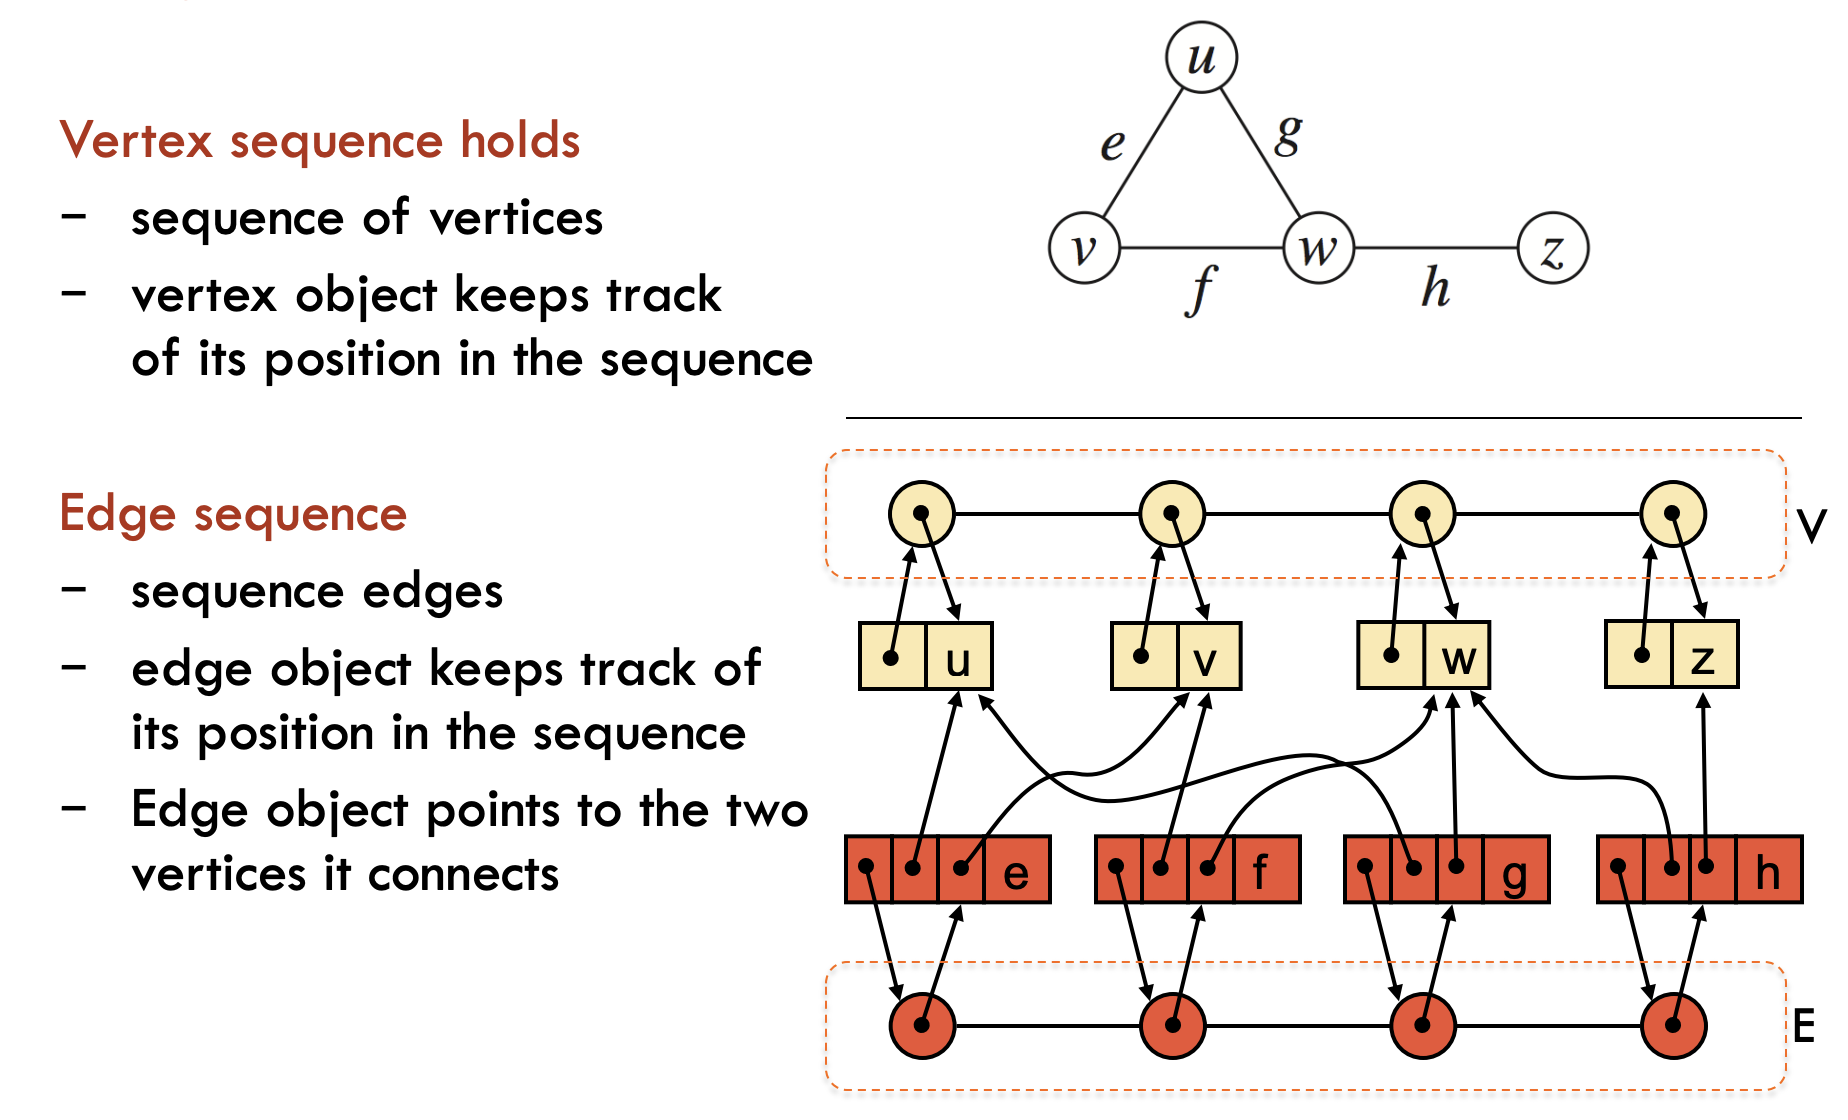
\includegraphics[width=\textwidth]{image13.png}

\subsection{Adjacency List}
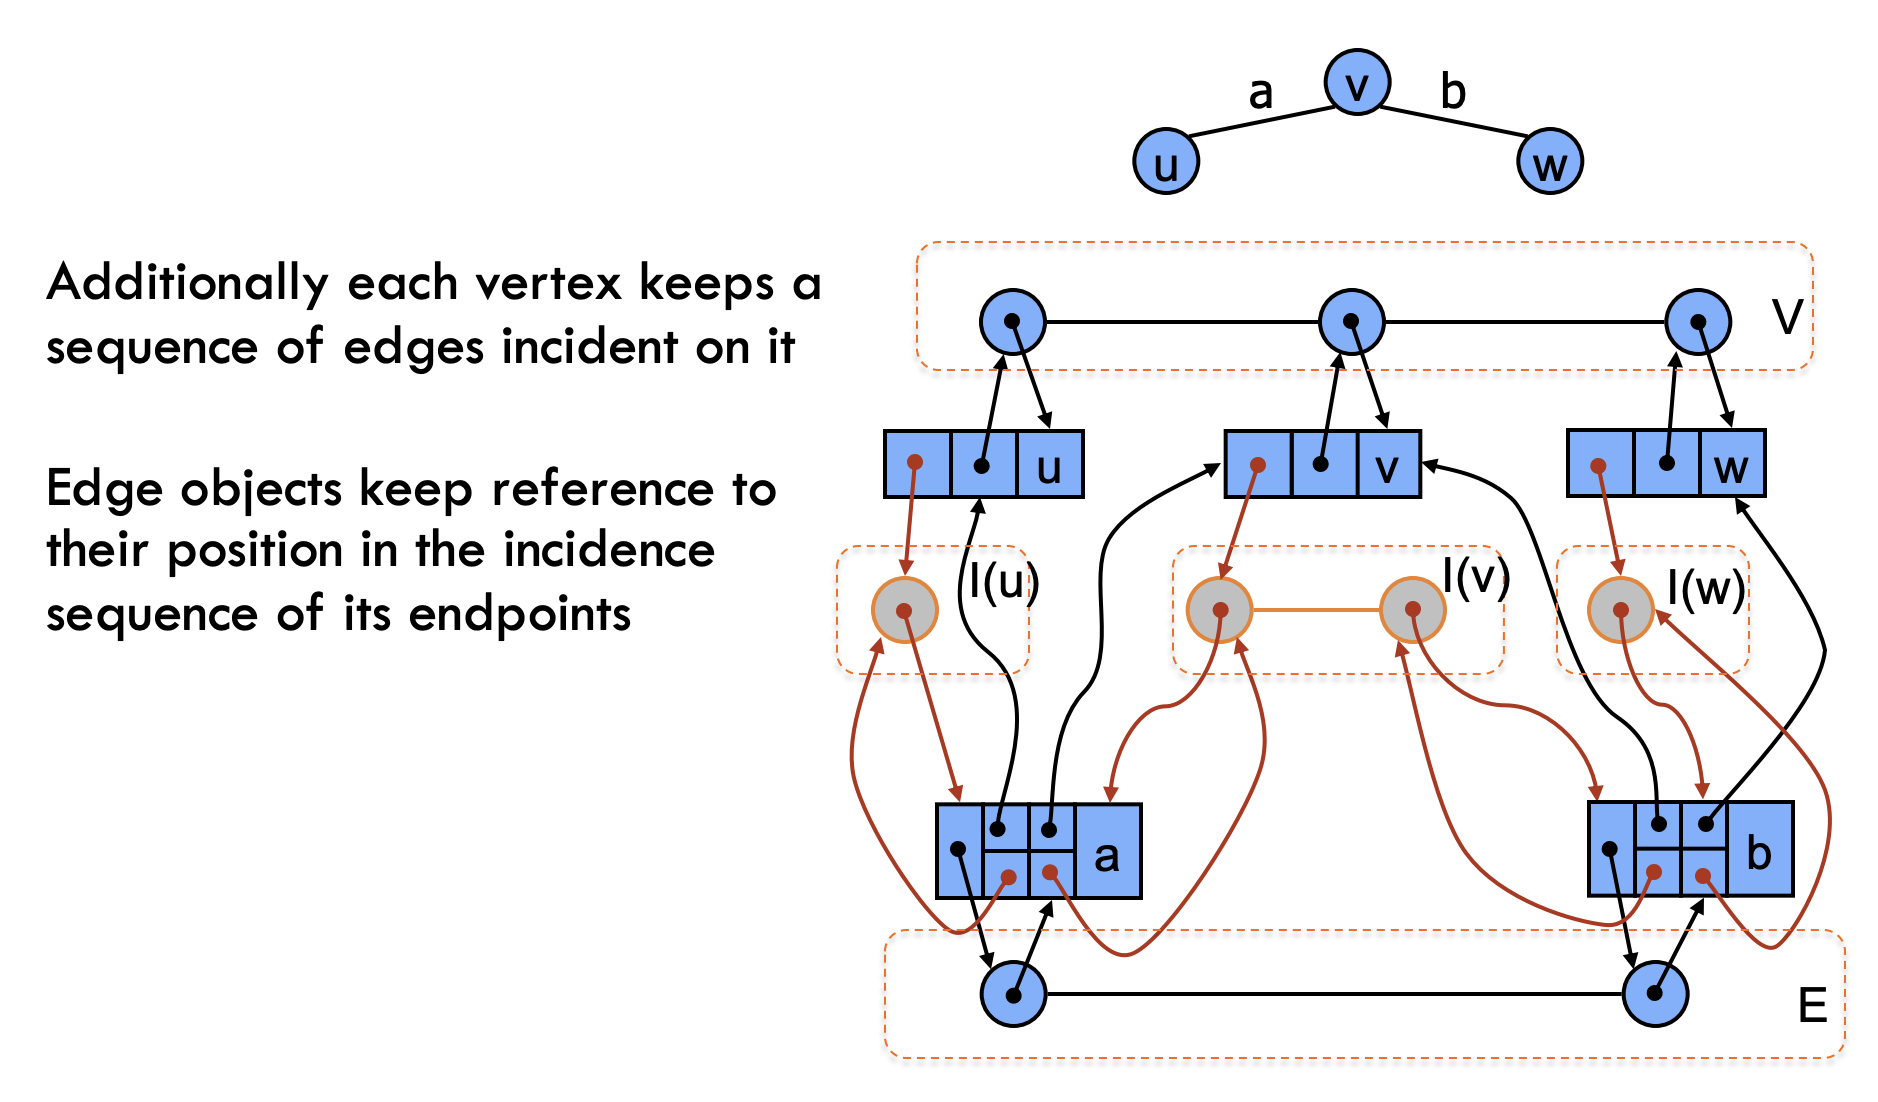
\includegraphics[width=\textwidth]{image14.png}

\subsection{Adjacency Matrix Structure}
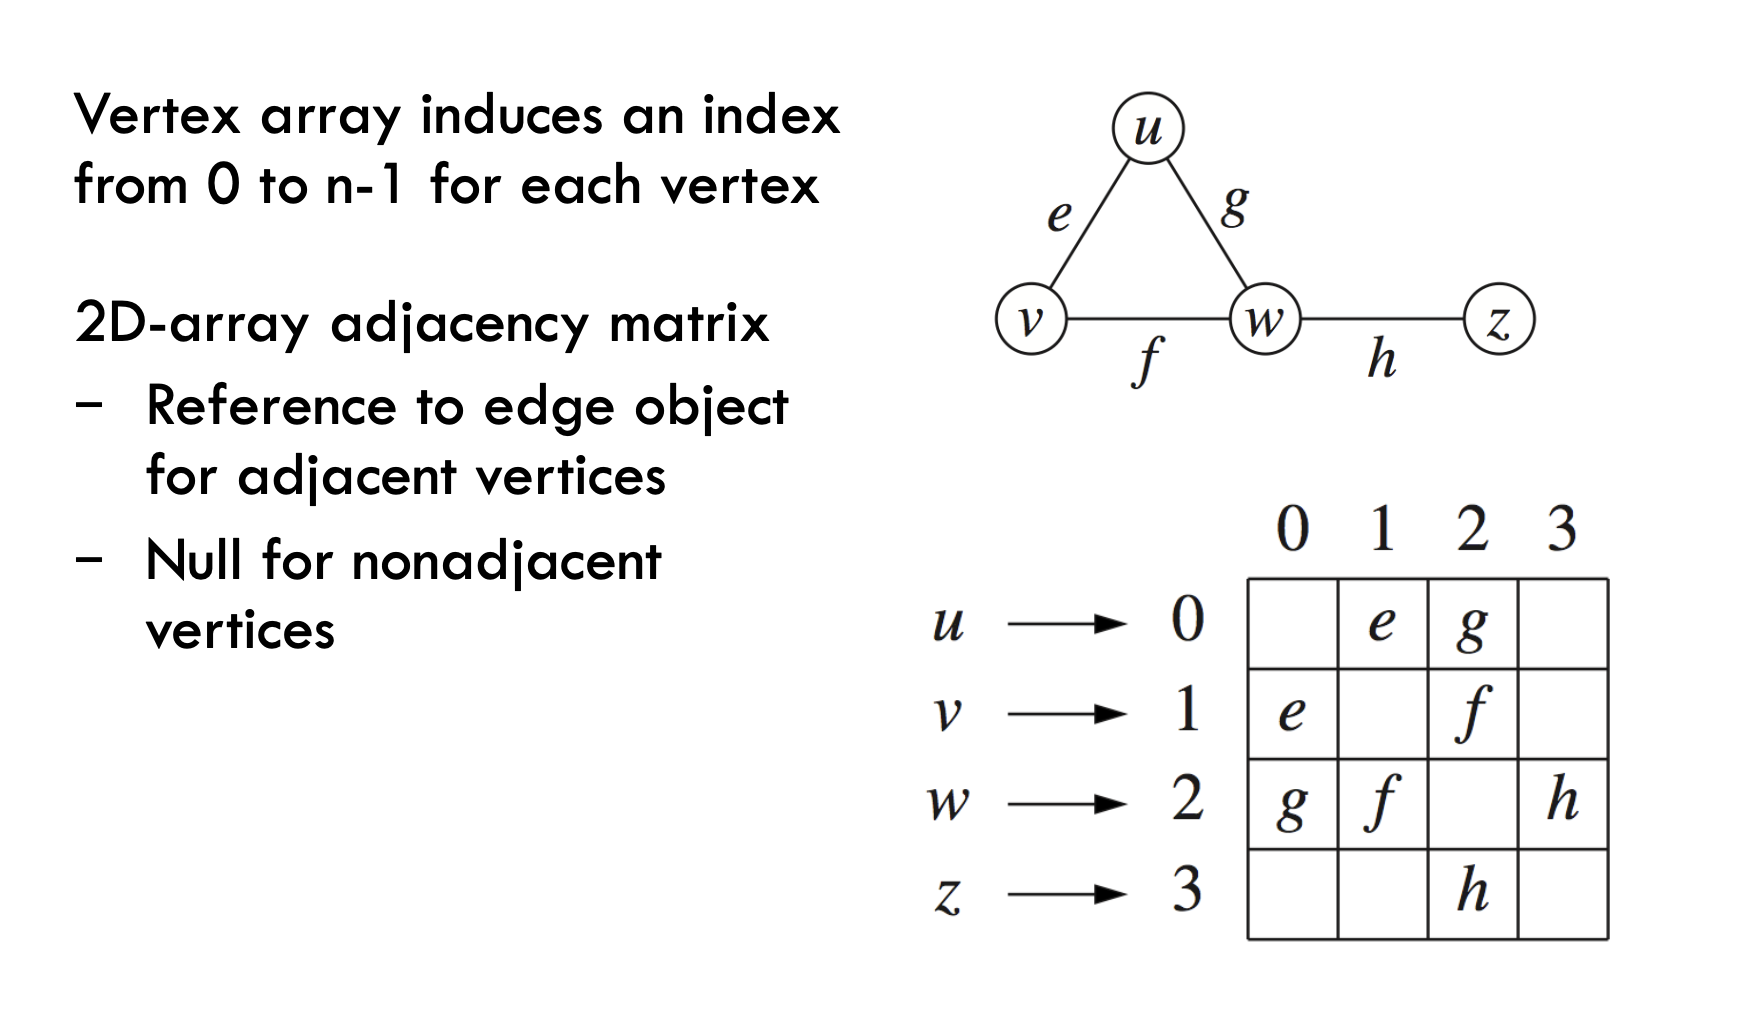
\includegraphics[width=\textwidth]{image15.png}

\subsection{Asymptotic performance}
\begin{tabular}{|l|l|l|l|}
  \hline
  \rowcolor{myBlue}
  \color{white}{\textbf{No parallel edges/s-loops}} & \color{white}{\textbf{Edge List}} & \color{white}{\textbf{Adjacency List}} & \color{white}{\textbf{Adjacency Matrix}} \\
  \hline
  Space  & O(n + m) & O(n + m) & O($n^2$) \\
  \hline
  incidentEdges(v) & O(m) & O(deg(v)) & O(n) \\
  \hline
  getEdge(u, v) & O(m) & O(min(deg(u), deg(v))) & O(1) \\
  \hline
  insertVertex(x) & O(1) & O(1) & O($n^2$)\\
  \hline
  insertEdge(u, v, x) & O(1)  & O(1)  & O(1) \\
  \hline
  removeVertex(v) & O(m) & O(deg(v)) & O($n^2$)\\
  \hline
  removeEdge(e) & O(1) & O(1) & O(1)\\
  \hline
\end{tabular}

% Section 3  ----------------------------------------------------------------------------------------
\section{Depth-First Search (DFS)}
This strategy tries to follow outgoing edges leading to yet unvisited vertices whenever possible, and 
backtrack if “stuck.” If an edge is used to discover a new vertex, we call it a DFS edge, otherwise we 
call it a back edge. The DFS edges form a spanning tree of the connected component being explored.
\begin{pseudo}
  \I \DEF{DFS}{G} \comment{Total run time is O(n + m)}
  \I \1 \for{u in G.vertices()} \comment{Set things up for DFS: O(n)}
  \I \2 visited[u] \assign false
  \I \2 parent[u] \assign null
  \I \1 \for{u in G.vertices()} \comment{Visit all vertices: O(n) not counting DFS\_Visit}
  \I \2 \IF{not visited[u]}
  \I \3 DFS\_Visit(u)
  \I \1 \return{parent}
\end{pseudo}
\begin{pseudo}
  \I \DEF{DFS\_Visit}{u} \comment{O(deg(u)). Total runtime: O(m)}
  \I \1 visited[u] \assign true
  \I \1 \for{v in G.incidentEdges(u)} \comment{Check out all neighbors of u}
  \I \2 \IF{not visited[v]}
  \I \3 parent[v] \assign u
  \I \3 DFS\_Visit(v)
\end{pseudo}
Let Cv be a connected component of v in our graph G. The DFS\_Visit visits all vertices in Cv
before returning to the outer loop. Edges \{(u, parent[u]): u in Cv\} form a spanning tree of C.
Edges \{(u, parent[u]): u in V\} form a spanning forest of G.

\vspace{10pt}
DFS runs in O(n + m). It can also solve other graph problems in this time. For example, it can 
find a path between two given vertices, if any, find a cycle in the graph, test whether a graph 
is connected, compute connected components of a graph and compute a spanning forest of a graph.

\subsection{Cut edges}
In a connected graph G=(V, E), we say that an edge (u, v) in E is a cut edge if (V, E / {(u, v)}) 
is not connected. The cut edge problem is  to identify all cut edges. We can solve this problem 
by running DFS on G. Trivial O(m2) time algorithm: For each edge (u,v) in E, remove (u,v)
and check using DFS if G is still connected, put back (u,v). Better O(nm) time algorithm: Only test 
edges in a DFS tree of G. Way to do it in O(n + m) but we don't know how to do it yet.

% Section 4  ----------------------------------------------------------------------------------------
\section{Breadth-First Search (BFS)}
This strategy tries to visit all vertices at distance k from a start vertex s before visiting vertices 
at distance k + 1:
\begin{itemize}
  \item L0 = {s}
  \item L1 = vertices one hop away from s
  \item L2 = vertices two hops away from s but no closer
  \item k = vertices k hops away from s but no closer
\end{itemize}
\begin{pseudo}
  \I \DEF{BFS}{G, s} \comment{Total run time is O(n + m)}
  \I \1 \for{u in G.vertices()} \comment{Set things up for BFS: O(n)}
  \I \2 visited[u] \assign false
  \I \2 parent[u] \assign null
  \I \1 seen[s] \assign true
  \I \1 layers \assign []
  \I \1 current \assign [s]
  \I \1 next \assign []
  \I \1 \while{current is not empty} \comment{O(m)}
  \I \2 layers.append(current)
  \I \2 \for{u in current} \comment{iterate over current layer}
  \I \3 \for{v in G.incidentEdges(u)} \comment{iterate over neighbors of u}
  \I \4 \IF{not seen[v]}
  \I \5 seen[v] \assign true
  \I \5 parent[v] \assign u
  \I \5 next.append(v)
  \I \2 current \assign next \comment{update current and next layer}
  \I \2 next \assign []
  \I \1 \return{layers, parent}
\end{pseudo}

\newpage
\subsection{BFS Properties}
\begin{itemize}
  \item Let $C_v$ be the connected component of $v$ in our graph $G$.
  \item Fact: BFS($G$, $s$) visits all vertices in $C_s$.
  \item Fact: Edges $\{(u, \text{parent}[u]): u \in C_s\}$ form a spanning tree $T_s$ of $C_s$.
  \item Fact: For each $v$ in $L_i$, there is a path in $T_s$ from $s$ to $v$ with $i$ edges.
  \item Fact: For each $v$ in $L_i$, any path in $G$ from $s$ to $v$ has at least $i$ edges.
  \item Fact: Assuming adjacency list representation we can perform a BFS
  traversal of a graph with n vertices and m edges in O(n+m) time
  \item Fact: Assuming adjacency matrix representation we can perform a
  BFS traversal of a graph with n vertices and m edges in O($n^2$) time
\end{itemize}

\subsection{BFS Applications}
BFS can be used to solve other graph problems in O(n + m) time. For example, it can
find the shortest path between two given vertices, find a cycle in a graph,
test whether a graph is connected or compute a spanning tree of a graph (if connected).

% Section 5  ----------------------------------------------------------------------------------------
\section{Terminology}

\subsection{Undirected graphs}
\begin{minipage}[l]{0.6\textwidth}
  \begin{itemize}
    \item Edges connect endpoints (e.g., W and Y for edge f)
    \item Edges are incident on endpoints (e.g., a, d, and b are incident on V)
    \item Adjacent vertices are connected (e.g., U and V are adjacent)
    \item Degree is the number of edges on a vertex (e.g., X has degree 5)
    \item Parallel edges share the same endpoints (e.g., h and i are parallel)
    \item Self-loop have only one endpoint (e.g., j is a self-loop)
    \item Simple graphs have no parallel or self-loops
  \end{itemize}
\end{minipage}
\begin{minipage}[r]{0.39\textwidth}
  \raggedleft
  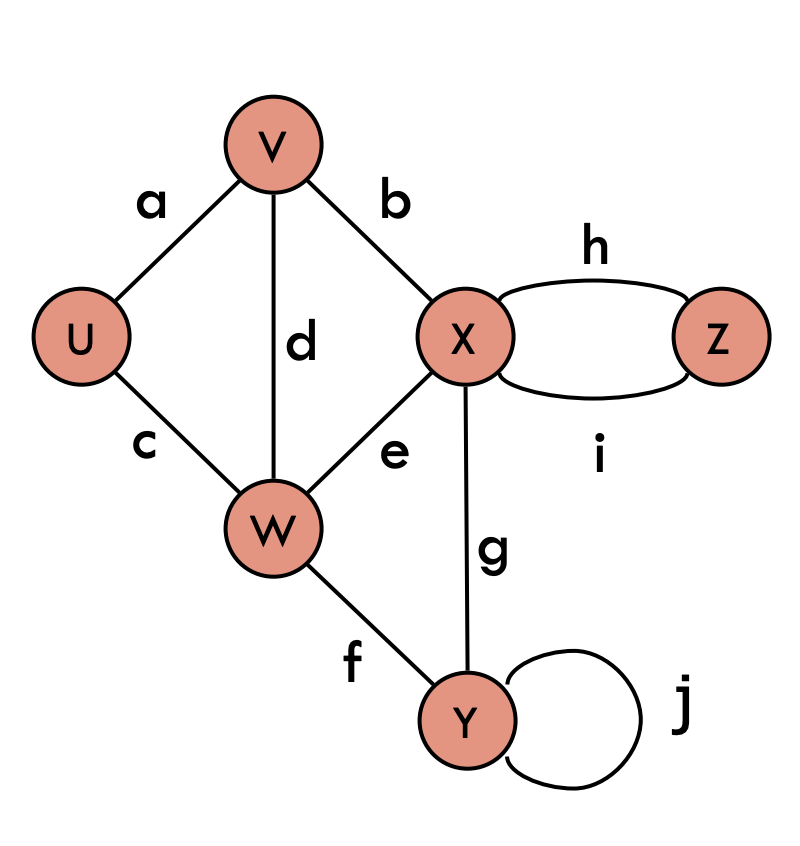
\includegraphics[width=\textwidth]{image16.png}
\end{minipage}

\subsection{Directed graphs}
\begin{minipage}[l]{0.6\textwidth}
  \begin{itemize}
    \item Edges go from tail to head (e.g., W is the tail of c and U its head)
    \item Out-degree is the number of edges out of a vertex (e.g., W has out-degree 2)
    \item In-degree is the number of edges into a vertex (e.g., W has in-degree 1)
    \item Parallel edges share tail and head (e.g., no parallel edge on the right)
    \item Self-loop have the same head and tail (e.g., X has a self-loop)
    \item Simple directed graphs have no parallel or self-loops, but are allowed to have antiparallel loops like f and a
  \end{itemize}
\end{minipage}
\begin{minipage}[r]{0.39\textwidth}
  \raggedleft
  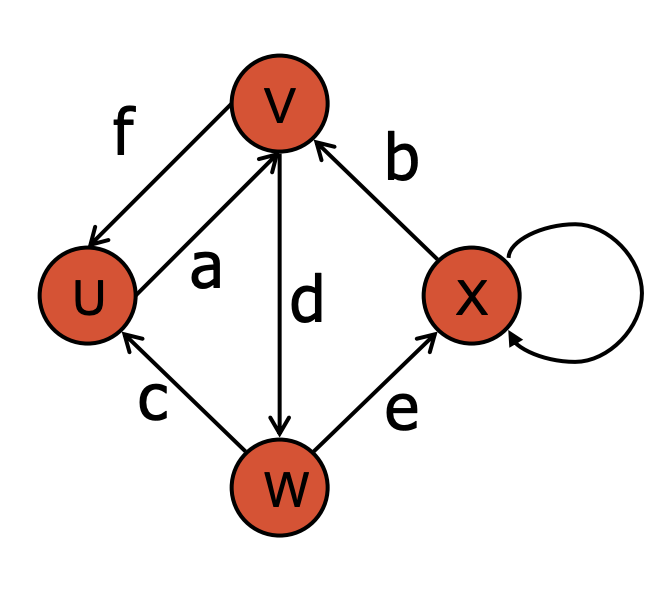
\includegraphics[width=\textwidth]{image17.png}
\end{minipage}

\end{document}

% Section 6  ----------------------------------------------------------------------------------------